\section{Introduction}

Around 2014, Generative Adversarial Networks, a type of neural network designed by Ian Goodfellow and his team \cite{goodfellow2014generative}, was introduced. The next year, Batch Normalization \cite{ioffe2015batch} and the definition of Residual Networks \cite{he2015deep} was born. These, amongst many more discoveries up until today allowed neural networks to deeper, more efficiently, and with much better results.

One paper from 2015 \cite{denton2015deep} shows outstanding -- for the time -- results in terms of image generation using GANs. From a very low quality image, the network is able to generate a completely new image, either reconstructing the original, or coming up with its own interpretation of the available data (Figure \ref{fig:eyescream}). The same year, another team in Toronto developed a neural network that could generate images from a natural language text description (Figure \ref{fig:gen_attention}). This was merely the start of the GAN revolution.

GANs allow the use of parameters that can be tuned to generate specific variants of the same output image. An example is the image of the face of a person, that smiles or frowns, according to a given parameter, or turns its head left and right, or has glasses on or off.

These advancements looked great, as they served to push the advancements in the field much forward. In the following years, more and more papers regarding GANs started to show up, highlighting the immense potential that this neural network architecture provided. As the development in this field progressed, more discoveries were made, and higher quality images could be reproduced.

In the following sections we are going to discuss what is realistic image generation more in detail, why it is a problem in the modern society, and what are possible consequences.

\begin{figure}
    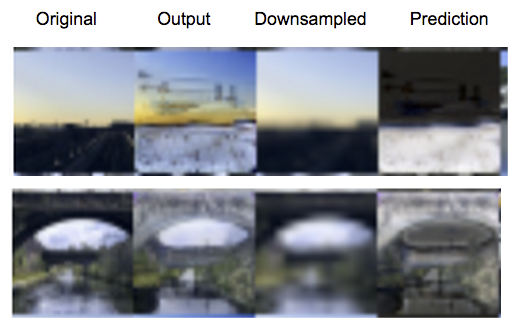
\includegraphics[width=\linewidth]{00_Introduction/eyescream_predicted16.png}
    \Description[Skyline and bridges, generated by Eyescream (2015)]{Skyline and bridges, generated by Eyescream (2015)}
    \caption{Skyline and bridges, generated by Eyescream (2015)}
    \label{fig:eyescream}
\end{figure}

\begin{figure}
    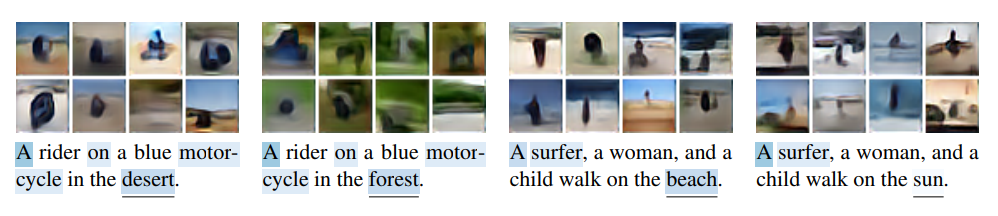
\includegraphics[width=\linewidth]{00_Introduction/gen_from_captions.png}
    \Description[Example of most attended words while changing the background in the caption]{Example of most attended words while changing the background}
    \caption{Example of most attended words while changing the background}
    \label{fig:gen_attention}
\end{figure}
